\documentclass[12pt]{article}

\newcommand\tab[1][1cm]{\hspace*{#1}}

\usepackage{times}
\usepackage{amsmath}
\usepackage{latexsym}
\usepackage{fullpage}
\usepackage{graphicx}
\usepackage{amsfonts}
\usepackage[dvipsnames]{xcolor}

\graphicspath{ {./images/} }

\newcommand{\NOT}{\neg}
\newcommand{\AND}{\wedge}
\newcommand{\OR}{\vee}
\newcommand{\XOR}{\oplus}
\newcommand{\IMPLIES}{\rightarrow}
\newcommand{\IFF}{\leftrightarrow}
\newcommand{\E}{\exists}
\newcommand{\A}{\forall}

\setlength{\parskip}{.1in}

\renewcommand{\baselinestretch}{1.1}

\begin{document}

\begin{center}

{\bf
CSCE 313\\
Quiz 2\\
Jeffrey Xu\\
527008162\\
09/18/20\\
}

\end{center}

{\bf 1.} [5 pts] While implementing the process state diagram, what is the problem of having only 1 queue for all blocked processes waiting for all events? What is the solution to this problem? Describe with an example.

The issue of having one queue is that is cannot handle different types of events. If a queue with a bunch of different processes waiting for different I/O events has a process at the front that is waiting for a keyboard interrupt but currently an audio I/O hits, then the queue can't really process the event that is waiting for the audio I/O as it isn't in the front. The queue is essentially a priority queue but with an undefined priority. The only way for having one queue is to have an oracle that can see into the future and assign priorities based on which I/O event will occur first. However, since we do not have the ability to time travel or predict the future with any more accuracy than a man throwing darts at a board while blindfolded, we must think of a more clever solution to our issue. 

The solution to this is to have queues for every single type of I/O. This takes away the "priority" sense of the queue and allows processes to be handled with other similar processes. Now, given our original queue, there is a queue for keyboard interrupt and another separate queue for audio I/O. If there is an audio I/O interrupt, the first element in the audio queue will get popped off and sent to the next state for processing. This allows the blocking mechanism to still work in $O(1)$ without too much overhead while still using the same amount of space. 

{\bf 2.} [25 pts] Assume the following processes A, B, C are loaded in memory of a system that uses both multiprogramming (MP) and timesharing (TS) techniques. These processes have 15, 7, and 13 instructions respectively. Also assume that the dispatcher lives at address 100 in memory and spans 4 instructions (i.e., 100-103). The time quantum is long enough for exactly 5 instructions.

The following table shows only instruction addresses in the memory with I/O requests labelled, along with the duration of these I/O operations in terms of CPU instructions. Although I/O operations do not take CPU instructions, the durations means that the I/O operations will finish by the time the corresponding number of CPU instructions execute.

Please draw one possible trace of these 3 processes running together in the CPU. Use page 14-15 of Lecture 3 for reference. You may skip the first invocation of the dispatcher to decide the first process to run in the CPU. 

\begin{center}
\begin{tabular}{| c | c | c |}
\hline
{\bf Process A} & {\bf Process B} & {\bf Process C}\\
\hline\hline
5000 & 8000 & 12000\\
\hline
5001 & 8001 & 12001 (I/O, takes 3 ins.)\\
\hline
5002 & 8002 & 12002\\
\hline
5003 & 8003 (I/O, takes 7 ins.) & 12003\\
\hline
5004 (I/O, takes 6 ins.) & 8004 & 12004\\
\hline
5005 (I/O, takes 4 ins.) & 8005 & 12005\\
\hline
5006 & 8006 & 12006 (I/O, takes 1 ins.)\\
\hline
5007 & & 12007\\
\hline
5008 (I/O, takes 5 ins.) & & 12008 (I/O, takes 2 ins.)\\
\hline
5009 & & 12009\\
\hline
5010 & & 12010\\
\hline
5011 & & 12011\\
\hline
5012 & & 12012\\
\hline
5013 & & \\
\hline
5014 & & \\
\hline
\end{tabular}
\end{center}

{\bf 3.} [5 pts] What is the difference between the "New" state and the "Ready to Run" state in the process diagram?

{\bf 4.} [5 pts] Is a transition from the "Blocked" state to directly to the "Exit" state possible in the process state diagram? How?

{\bf 5.} [10 pts] Assume that the following physical memory is full with already allocated 5 pages as shown below (i.e., it is 20KB in capacity). Describe what happens if process 2 wants to allocate and use another page. What changes in the page tables and the physical memory? 

\begin{center}
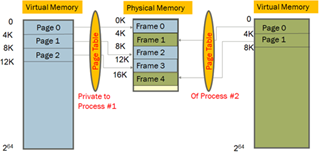
\includegraphics[width=8cm, height=4cm]{313Quiz2P5}
\end{center}

{\bf 6.} [25 pts] Draw the Descriptor Table (DT) and the File Table (FT) for each possible process just after executing the lines 2, 5 and 10 and explain what you see in the standard output and {\bf file.txt} along the way. 

\begin{center}
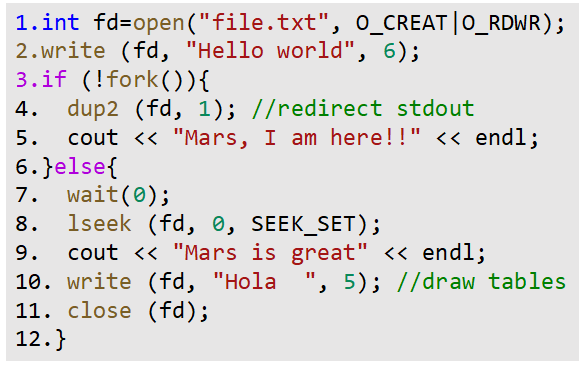
\includegraphics[width=8.5cm, height=6cm]{P6}
\end{center}

{\bf 7.} [25 pts] Please explain the output of the following program using a process tree diagram as shown in Lecture 4 page 23. Assuming the main process's ID is 1000, explain the order of process creation (in fact, the number itself should show what order the processes are created). Also explain what you see in the standard output. Are different outputs possible for this program? Why or why not? 

\noindent
{\color{violet} for} ({\color{blue} int} i={\color{Green}0}; i$<${\color{Green}4}; i++) \{\\
\tab{\color{blue}int} cid = {\color{RawSienna}fork}();\\
\tab{\color{violet}if}(i$<${\color{Green}2})\\
\tab\tab{\color{RawSienna}wait}({\color{Green}0});\\
\tab cout $<<$ {\color{Maroon}"ID="} $<<$ {\color{RawSienna}getpid}() $<<$ endl;\\

\end{document}